% Some commands used in this file
\newcommand{\product}{\textit}

\chapter{Material and Methods}

\section{General information}
All the liquids that would be be in contact with the cell, were pre-warmed in water-bath to limit cold-exposure. Unless specifically stated otherwise, we worked under sterile conditions. By courtesy of Dr. Ulrich Blache, we had access to human bone-marrow derived mesenchymal stem cells from pseudonymized patients. Incubation parameters are kept constant at 37 \degC{} and 5\% CO2 in humidified air.

\section{Cell Culture And Passaging}

Cells are grown in growth medium under sterile conditions. Nunc\texttrademark{} EasYFlask\texttrademark{} Cell Culture Flasks with filters (ThermoFisher) were used for growing the cells. The media was changed every three days. Passaging was done at 80\% confluence using the following standard TE-protocol. First, the cells are generously washed with PBS. Second, 2ml Trypsin-EDTA (TE, maduzi) is added and the cells incubated for 3-10 minutes. Then, add 10ml MEM\textalpha{} with 10\% FBS and transfer cell solution to 15ml Falcon Tube. Centrifuge for 5 minutes at a speed of 500 rcf. Next, discard the supernatant and resuspend the cells in Growth Medium and seed according to application with typical seeding density being 10\textsuperscript{6} Cells / 75 cm\textsuperscript{2}. 
Growth Medium consist of ROTI\textregistered{} Cell Eagle's MEM\textalpha{} with nucleosides and stable l-glutamin(ROTH), 10\% FBS (heat-inactivated, Thermo Fisher) and 5ng/ml Growth Factor FGF-2 (PeproTech).

\section{Retroviral Transduction}
From 100\% confluent cells, seed approximately 800'000 cells in T25 according to standard protocol. On the next day, remove medium and add 1ml of Polybrene Medium (MEM\textalpha{}, 5\% FBS, 1\mul{}/ml Polybrene (Sigma-Aldrich)). From here onward, Biosafety Level (BL) 2 measures were applied. Carefully, add 1ml of virus construct to corresponding flask. Incubate at 4 \degC for two hours, followed by addition of 3ml Compensation-Medium (3ml MEM\textalpha{}, 5\% FBS, 1\mul{}/ml Polybrene and 8 ng/ml FGF-2), after which the cells were incubated over night. Then remove medium and add 5ml standard Growth Medium. On the next day, split 1:3.5 depending on confluence. On the day after, start selection by removing old medium and adding Selection Medium (Growth Medium + 3\textmu{}g/ml Puromycin (Thermo Fisher Scientific)) and incubating the cells for 72 hours. After incubation, pre-validate knock-out with comparing negative control (expected: low viability) to KO-cell-line (expected: high viability) under light microscope. Over the next days, the cells are split another three times until the virus particles are neutralized and the BL restrictions can be relaxed from BL2 to BL1. Quality of knock-out is definitely assessed with Western Blot (Protein) and qRT-PCR (mRNA). Freeze or cultivate according to need. 

\begin{figure}
    \centering
    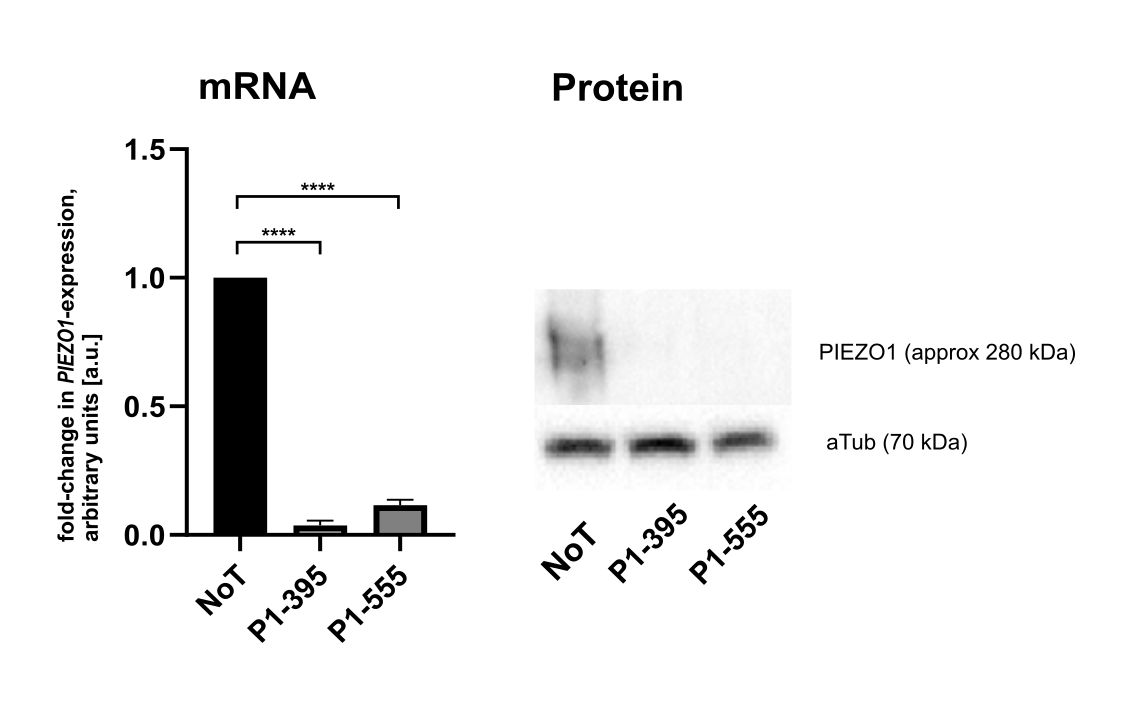
\includegraphics[width=\linewidth]{Piezo1KO_Verification_WBandPCR.png}
    \caption{Validation of successful knockout on mRNA (left) and Protein (right) level with housekeeping genes being RPL13A}
    \label{fig:KO-Verification}
\end{figure}

\section{RNA Analysis}
\subsection{RNA Extraction}
This was prepared in open space. Cells were either directly lysed in-well after PBS washing or lysed in the tube, after being collected from well and washed with PBS. Lysis-Buffer was supplemented with 1\% \textbeta-mercaptoethanol. The whole cell lysate was either frozen for later processing or directly processed. When freezing the lysate, the tube is shock-frozen in liquid nitrogen before transferred to -80 \degC freezer. When processing, the PureLink PCR Micro Kit (\product{Thermo Fisher, CN: K310250}) following manufacturer's protocol was used, dissolving the RNA in the final step with 20\mul{} of RNase-free Water (BioConcept). The final concentration of the sample was assessed using the Qubit RNA HS Assay Kit (ThermoFisher) with a new calibration each time a new working solution was prepared.

\subsection{Reverse Transcription}
This was prepared in open space. Unless stated otherwise, 300ng of RNA was transcribed per 40\mul{} total reaction volume using the High-Capacity cDNA Reverse Transcription Kit (Thermo Fischer) following supplier's instructions. \myworries{Insert program specification of Cindy Thermal Cycler (MasterCycler, Eppendorf)}. Samples were either stored at -20 \degC or immediately downstream processed. 

\subsection{Quantitative Real-Time PCR Analysis}
All real-time PCR analyses were performed on an StepOnePlus ThermoCycler real-time PCR system (Applied Biosystems) with a 96-well plate as a carrier device. Each reaction well contained a reaction volume of 2\mul{} sample cDNA and 8\mul{} Primer-specific PCR MasterMix (KAPA PROBE FAST MasterMix (KAPA Biosystems), TaqMan\textregistered{} Primer (ThermoFisher) and RNase-free Water). The C\textsubscript{t}-value (cycle threshold) value for each gene was determined using the automated threshold analysis in the StepOnePlus device. Data was evaluated using the comparative C\textsubscript{t}-Method with GAPDH and RPL13A as housekeeping genes.

Investigated gene products and corresponding primers used are (Product Number TBA): 
\begin{itemize}
\item COL1
\item COL3
\item FN1
\item IL6
\item IL11
\item ALPL
\item RUNX1
\item SPP1
\item GAPDH 
\item RPL13A
\end{itemize}

\section{Protein Analysis}
\subsection{Preparation}
After washing the cells with PBS, 0.5ml of TE(1X) was added to each well, after which the cells where incubated for 3-8 minutes. As to maximize yield, we additionally employed a scraping protocol. 1ml of MEM\textalpha{} + 10\% FBS is added per well and the cells gently scraped off using a cell scraper (Sarstedt). Then transfer the cells into a eppendorf tube, followed by a RT centrifugation step at 2'000 rcf for 5 minutes after which the supernatant is discarded. Then the tube is filled with 1.5ml of PBS and the centrifugation step including the discarding of supernatant repeated. Finally, the tubes are shock-frozen in liquid nitrogen before transferring them to a -80 \degC freezer for storage. When processing, the protein samples, the whole cell pellet was dissolved in 20\mul{} of \textsc{Ripa}-Buffer (Sigma-Aldrich). After incubation on ice for 20 minutes, during which each sample was vortexed three to four times, the samples are 4 \degC centrifuged at maximum speed for 10 minutes. For further processing, only the supernatant is used. Measure protein concentration of all samples by employing the DC\texttrademark{} Protein Assay (BioRad), following the manufacturer's protocol and comparing it to the personal standard curve. Then protein concentration was normalized while maximized (i.e. dilute with RIPA all samples to match concentration of lowest concentration sample). 

\subsection{Western Blotting}
In new tube Laemmli-Buffer(6X) (BioRad) and sample was mixed to a final volume of 15\mul{}, then  vortexed 5 seconds and then cooked for 4-8 minutes at 95 \degC in ThermoCycler (i.e. cooking), where each tube contained the same amount of protein. Then the sample was loaded onto a 4–15\% Mini-PROTEAN TGX Stain-Free Protein Gel (BioRad) and resolved by electropphoresis at constant current of 35mA. Then the gel is wet-transferred onto PVDF Membrane (BioRad) using Trans-Blot Turbo Transfer System (BioRad). The membrane was then blocked in 5 wt\% low fat dry-milk (Migros) in TBST (i.e. blocking solution) for 1 hour. This is followed by incubation primary antibody either for 2 hours at room temperature or 14 hours at 4 \degC{} under constant shaking. After 3 times 10min washing in TBST, it is incubated in the matching secondary antibody, which is conjugated to HRP. Every time before immersion medium changes, the membrane was washed three times in TBST for 10 minutes. SuperSignal Ultra/Femto  detection reagents (Pierce) were used for visualization. The exposure time were manually set, to accomodate maximum signal while avoiding saturation. Only after successful imaging of the protein of interest, incubation for housekeeping protein was started. Quantification was done manually with Fiji (version 2.0.0-rc-69, Java 1.8) with the analysis workflow describde elsewhere \cite{Miller2010}.



\begin{itemize}
    \item Primary Antibodies (TBA)
    \begin{itemize}
		\item AB 1
    \end{itemize}

 	\item Secondary Antibodies (TBA)
    \begin{itemize}
		\item AB 2
    \end{itemize}
\end{itemize}


\section{Chemical stimulation of \Piezo{} with \Yoda{}}
\label{sec:ChemicalStimulation}
Confluent cells were seeded on 6 well plates at concentration of 240'000 cells/well and kept serum starved for 8-14h in the incubator without additional FGF-2. \\
The intervention is initiated with a washing step, before 2.5ml of Intervention Medium (i.e. MEM\textalpha{} + 5\textmu{}M \Yoda (Sigma-Aldrich)) is added. Negative control samples were supplemented with MEM\textalpha{} only. The cells were then incubated for exactly 30 minutes, after which they are washed twice, before adding MEM\textalpha{} as culture medium and incubating cells until harvesting. RNA and Protein samples were collected after 0, 24, 48 and 72 hours using the respective standard protocol.\\ \cite{Morley2018} as for evidence for correct concnetration.

\section{Fluidic Shear Stress Model}
As the result of the Masters Thesis Project from Patrick Jäger, we have access to a flow chamber, which describes an device, that enables us to apply fluidic shear stress to cells in a fully controlled environment, with the only requirement of the cells being adherent. This flowchamber allows arbitrary choice of shear media, cell type and cellular alignment relative to flow, while leaving the researcher the opportunity to chose from either in-situ real-time calcium imaging, recultivation for additional steps or direct downstream processing.

\subsection{Flowchamber and seeding}
\label{sec:FluidicModel}
To produce the PDMS part of the flowchamber, firstly, 10 parts of silicone (SUPPLIER NAME) and 1 part of cross-linker (SUPPLIER NAME) are combined and vigorously mixed for 5 minutes using a single-use spatula. Then put in vacuum chamber that oscillates between 60 and 120 mbar to rid the gel of all bubbles. Put the gel in negative, metal form, then vacuum again. The form is then put on heating plate over night at 70 \degC{}. After the microscopy slides underwent plasma treatment for 4 minutes, we glue a stamp, on the slide using the silicon-crosslinker-mixture from earlier. Then we put them over night next to the metal form on a heating plate. On the next day, remove the PDMS stamps from microscopy slide, leaving behind PDMS grating. Decorate the stamps with Collagen-1 using Sulfo-SANPAH as a crosslinker. Proceed with separating the flowchamber pieces and punch entry point for syringe. Prepare glue by adding 3\mul of Platinum reagent (SUPPLIER and NAME) to 1g of silicon, mix for 3 minutes. Add 0.1g of Crosslinker, mix again for 5 minutes. Now glue PDMS-pieces on glass slide and put in oven at 45 \degC{} for 45 minutes. Either we stored them in the fridge or seed cells for an experiment on the next day.\\
For seeding, we work sterile in the cell culture lab. Flowchambers are sterilised through generous use of 80\% EtOH (including flushing of chamber). Flush the chamber twice with PBS. Prepare cell solution of 1 Mio Cells/ml in Growth Medium. Add 70 \mul{} of cell solution per flowchamber. After 45 minutes of incubation, flush the chamber with 200\mul{} of Growth Medium to remove non-adherent cells, while making sure to avoid cell-air contact. Put in incubator over night with the experiment scheduled on the next day.

\subsection{Fluorescence staining and imaging}
In 500\mul{} of pre-incubated Growth Medium dissolve 2\mul{} Fluo-4 (ThermoFisher) (i.e. Staining Medium). Add 200\mul{} of Staining Medium per flowchamber and let it incubate 2h until the start of the experiment. 
Minimise photobleaching by decreasing unnecessary light exposition. In a dark microscopy room, connect the flowchamber with a syringe that is fixed on the NemeSys syringe system (Cetoni). The syringe holds artifical cerebrospinal fluid (ACSF),depending on the experiment mixed according to standard or calcium-free protocol, whose respective ingredients is described in the appendix (\myworries{TODO!}). The flow protocol used throughout this project incorporates a small continous flow with a stark increase in flow rate for a total of 5s. Imaging was done with excitation wavelength of \textlambda{} = 488 nm. Imaging protocol in LiveAcquisition (v1.2.2, TILL Photonics) over 120 seconds per measurement incorporating a Z-stack of five layers to account for shear-mediated displacement of cell, which lead to a total of 600 pictures. Reduce image to two dimensional Z-projection with average intensity method.  \\
Note that in the extracellular Ca-influx experiment we flushed the flowchamber for 12 minutes (equivalent to 2.4ml medium) with normal ACSF in between measurements of the same cell patch.


\subsection{Processing and evaluation}

The time-trace of brightness levels of individually segmented cells was done using a workflow implemented in R and ImageJ scripts implemented by Patrick Jäger, using ImageJ (v1.52p) and R Studio. Simplified the workflow consisted of following steps:

\begin{itemize}
	\item Segmentation of cells using the first frame, feeding them in the ROI Manager
	\item Record brightness levels over the whole measurement
	\item Normalization of each brightness for each cell individually using the average of first 15 frames (Leading to one table per flowchamber with size Frames$\times$Cells)
	\item Pooled data of all flowchambers belonging to the same patient in one table
	\item Reduce to matrix of size Frames$\times$3, with columns being Cell Count, Average Signal and Standard Deviation
	\item Maximum Value was found using maxVal-Function over the whole measurement interval
\end{itemize}

Important details are that per recording there was exactly one normalization, leading to seemingly discontinuous jumps in the concatenated measurements of changing flushing medium. Also, we did not manually adjust ROIs. 



